\chapter{Background}

Filesystems are collections of methods and data structures that an operating system uses to keep track of data on disks or partitions.Different operating systems uses different types of file systems like Windows uses NTFS and FAT32 file systems.Linux uses EXT4,EXT3,EXT2 etc.Earlier Android kernels used YAFFS2 file systems ,However newer Android kernels use EXT4 file systems.File systems atre implemented at kernel level.Implementing a new file system at the kernel level involves modifying the kernel source code and rebuilding it with the new file system support,This creates complexity which can be solved by implementing file system at the user level .
\section{Fuse(File system in User Space)}
\begin{figure}[H]
   
    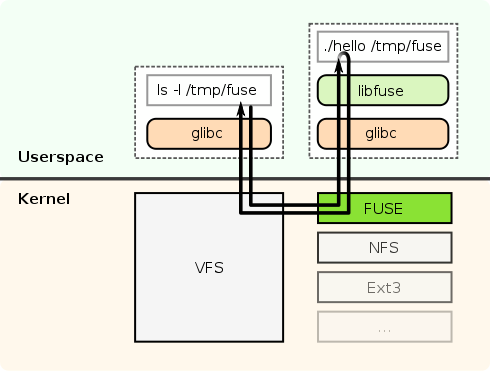
\includegraphics[width=0.7\textwidth ]{Figures/fig02/fuse}
    \caption{\href{https://en.wikipedia.org/wiki/Filesystem_in_Userspace}{Filesystem in Userspace }} 
  \end{figure}
FUSE (Filesystem in Userspace) is an interface for userspace programs to export a filesystem to the Linux kernel. The FUSE project consists of two components: the fuse kernel module  and the libfuse userspace library . FUSE is particularly useful for writing virtual file systems. Unlike traditional file systems that essentially save data to, and retrieve data from, mass storage, virtual filesystems do not actually store data themselves. They act as a view or translation of an existing file system or storage device. FUSE has a small kernel module  which plugs into the VFS layer in the kernel as a file system and then communicates with a user-level process that does all the work, using the FUSE library to communicate with the kernel module. IO requests from an application are redirected by the FUSE kernel module to this user level process for execution and the results are returned back to the requesting application.
\linebreak
A fuse file system is a user-space program that listens on a socket for file operations to perform and perform them. The fuse library(libfuse) provides the communication with the socket and passes the requests to the code.The callbacks are a set of functions to implement the file operations and a struct fuse\_operations contains pointers to them.\\




Necessary operations in fuse\_operation structure \cite{Writing_a_FUSE_Filesystem}\\
struct fuse\_operations \{
\begin{itemize}

\item  int (*getattr) (const char *, struct stat *);

\item int (*readlink) (const char *, char *, size\_t);

\item int (*getdir) (const char *, fuse\_dirh\_t, fuse\_dirfil\_t);

\item int (*mknod) (const char *, mode\_t, dev\_t);

\item int (*mkdir) (const char *, mode\_t);

\item int (*unlink) (const char *);

\item int (*rmdir) (const char *);

\item int (*symlink) (const char *, const char *);

\item int (*rename) (const char *, const char *);

\item int (*link) (const char *, const char *);

\item int (*chmod) (const char *, mode\_t);

\item int (*chown) (const char *, uid\_t, gid\_t);

\item int (*truncate) (const char *, off\_t);

\item int (*utime) (const char *, struct utimbuf *);

\item int (*open) (const char *, struct fuse\_file\_info *);

\item int (*read) (const char *, char *, size\_t, off\_t, struct fuse\_file\_info *);

\item int (*write) (const char *, const char *, size\_t, off\_t,struct fuse\_file\_info *);

\item int (*statfs) (const char *, struct statfs *);

\item int (*flush) (const char *, struct fuse\_file\_info *);

\item int (*release) (const char *, struct fuse\_file\_info *);

\item int (*fsync) (const char *, int, struct fuse\_file\_info *);

\item int (*setxattr) (const char *, const char *, const char *, size\_t, int);

\item int (*getxattr) (const char *, const char *, char *, size\_t);

\item int (*listxattr) (const char *, char *, size\_t);

\item int (*removexattr) (const char *, const char *);

\};

\end{itemize}

\begin{figure}[H]
   \centering
    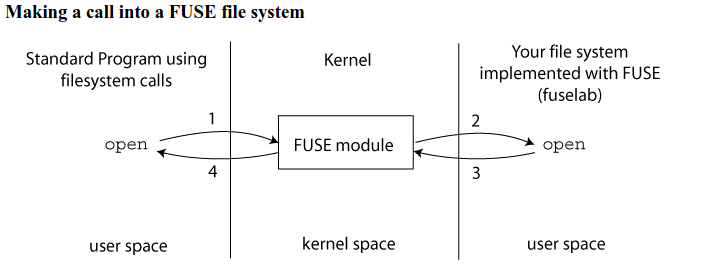
\includegraphics[width=0.7\textwidth ]{Figures/fig02/workingfuse}
    \caption{\href{https://www.cs.cmu.edu/~fp/courses/15213-s07/lectures/15-filesys/}{Making a Call in Fuse File System} } 
  \end{figure}


\textbf{Example of Fuse Filesystems:\cite{wiki:Filesystem_in_Userspace}} 
\begin{itemize}

\item \textbf{CloudStore (formerly, Kosmos filesystem):} By mounting via FUSE, existing Linux utilities can interface with CloudStore
\item \textbf{EncFS:} Encrypted virtual filesystem
\item \textbf{ExpanDrive:} A commercial filesystem implementing SFTP/FTP/S3/Swift using FUSE
\item \textbf{GDFS:} Filesystem which allows you to mount your Google Drive account on Linux.

\item \textbf{GlusterFS:} Clustered Distributed Filesystem having ability to scale up to several petabytes.
\item \textbf{GmailFS:} Filesystem which stores data as mail in Gmail.
\item \textbf{GVfs:} The virtual filesystem for the GNOME desktop.
\item \textbf{KBFS:} A distributed filesystem with end-to-end encryption and a global namespace that uses FUSE to create cryptographically secure file mounts.
\item \textbf{MooseFS:} An open source distributed fault-tolerant file system available on every OS with FUSE implementation (Linux, FreeBSD, NetBSD, OpenSolaris, OS X), able to store petabytes of data spread over several servers visible as one resource.
\item \textbf{NTFS-3G and Captive NTFS:} allowing access to NTFS filesystems.
\item \textbf{Sector File System:} Sector is a distributed file system designed for large amount of commodity computers. Sector uses FUSE to provide a mountable local file system interface.
\item \textbf{SSHFS:} Provides access to a remote filesystem through SSH.
\item \textbf{Transmit:} A commercial FTP client that also adds the ability to mount WebDAV, SFTP, FTP and Amazon S3 servers as disks in Finder, via MacFUSE.
\item \textbf{WebDrive:} A commercial filesystem implementing WebDAV, SFTP, FTP, FTPS and Amazon S3.
\item \textbf{WikipediaFS:} View and edit Wikipedia articles as if they were real files.
\item \textbf{Wuala:} A multi-platform, Java-based fully OS integrated distributed file system. Using FUSE, MacFUSE and Callback File System respectively for file system integration, in addition to a Java-based app accessible from any Java-enabled web browser.
\end{itemize}

\section{Cloudfs}
CloudFS will be developed using the file system in user-space (FUSE) toolkit. FUSE provides a framework for implementing a file system at user level.  CloudFS will be implemented  as user-level code that uses libfuse to communicate with  applications  and uses regular file system calls  to access the storage. By default, FUSE is multi-threaded, so multiple system calls from user applications can be running at the same time in the user-level process, allowing higher parallelism and  faster performance. Cloudfs can be used to mount cloud storage like dropbox, google drive and onedrive as local file system and any changes that are made in the local file system are syncronised with cloud storage. For example :
\begin{itemize}
\item WingFS, the universal cloud adapter, mounts the cloud service on the desktop.Storage services can be used  like a hard drive without the need for apps, specific folders, browser plug-ins and login processes.
\item Google Cloud Storage Fuse: It is an open source fuse adapter that allow us to mount Google cloud storage buckets as file systems on Linux or OS X systems. It also provides a way for applications to upload and download google cloud storage objects using standard file system semantics. It is written in Go language and hosted in github.
\item The Storage Made Easy Linux App Suite is comprised of an integrated Cloud Drive (that uses FUSE), a graphical Cloud File Explorer and also Sync tools to sync cloud files to/from the Linux desktop.
\item Drop-Fuse is a simple fuse based file system which is written in python and can mount the dropbox drive as local file system in Linux.


\end{itemize}
In our case We will be implementing the cloud fs below the android software stack in linux level and api's will be used synchronization and mounting a multitude of cloud storage services.
\section{Stealthfs via Rootkits}
When we  install a rootkit in that system we will be able to get administrator privileges whenever you want. Good rootkits can hide in compromised system, so that they can't be found by administrator. There are many ways to hide in a system.For example there are rootkits that replace some most important programs in system(ls, ps, netstat etc.) with modified versions of them that won't let administrator see that something's wrong. Although, such a rootkit is quite easy to detect. Other rootkits work as linux kernel modules. They work in kernel mode, so they can do everything they want. They can hide themselves, files, processes etc.\\
\linebreak
\bigskip 
Different types of Rootkits are explained below.
\subsection{User Level Rootkits}

User level rootkits are unprivileged and are stored outside of kernel memory
 space. They are user space code that patches or replaces existing applications to provide
 cover for malicious activities. User level rootkits replace system binaries, add malicious
 utilities, change configuration files, delete files, or launch malicious processes.For example, the Linux system program ‘ls’ could be changed so as to not reveal the
 presence of a malicious file in a directory. These rootkits, while effective, are easily
 detected by file system integrity and signature checking tools , therefore, most
 modern IDS software prevent these rootkits from being installed or can detect an active
 intruder.

\subsection{Kernel Level Rootkits}
Kernel level rootkits defeat such tools by directly modifying the operating system
 kernel. These rootkits modify the execution flow of kernel code to run their own payload.
 However, modifying the kernel in this way can drastically affect the stability of the
 system causing a kernel panic.

The simplest way to introduce code into a running kernel is through a Loadable
 Kernel Module (LKM) . LKMs add flexibility to an operating system by
 providing a means to add functionality without recompiling the entire kernel. Added
 functionality might include device drivers, filesystem drivers, system calls, network
 drivers, TTY line disciplines, and executable interpreters . Most modern UNIX-
like systems, including Solaris, Linux, and FreeBSD, use or support LKMs.
However, the kernel packaged with Android does not support LKMs by default. The
 kernel can be recompiled and installed on Android to add LKM support if physical access
 to the mobile is available. LKMs are very useful, but they also allow maliciously written
 kernel modules to subvert the entire operating system which can lead to a loss of control
 of the Linux kernel and consequently all the layers above the kernel . Kernel level
 rootkits typically subvert the kernel to hide processes, modules, connections and more to
 avoid detection. Particular techniques include hooking system calls, direct kernel object
 manipulation (DKOM), run-time kernel memory patching, interrupt descriptor table
 hooking, and intercepting calls handled by Virtual File System (VFS). These techniques
 are discussed at a high level in this section.


\subsubsection{Hooking System Calls}
The kernel provides a set  of  interfaces or system calls by which processes running
 in user space can interact with the system. The applications in user space send requests
 through this interface and the kernel fulfills requests or returns an error. Hooking is a technique that employs handler function, called hooks, to modify
 control flow . A new hook registers its address as the location for a specific
function, so when that function is called the hook runs instead. Typically, a hook will call
 the original function at some point to preserve the original behavior. System calls can be
 hooked using a maliciously designed LKM to alter the structure of the system call table.

\subsubsection{Direct Kernel Object Manipulation (DKOM)}
Hooking the system write call allows a rootkit to hide from system binaries like
 ls, lsmod, and ps; even so, robust IDSs can still detect the existence by following the
 kernel structures. All operating systems store internal record-keeping
 keeping data in main
 memory . The Linux kernel is no exception and provides generic data structures
 and primitives to encourage code reuse by developers . These structures, that all
 programmers are familiar with, include linked lists, queues, maps, and binary trees.
 Altering the data in these structures to hide an attacker’s activity is called Direct Kernel
 Object Manipulation (DKOM).

\subsubsection{Interrupt Descriptor Table (IDT) Hooking}
An interrupt is an event that alters the sequence of instructions executed by the
 processor. When an interrupt occurs a system table called the Interrupt Descriptor Table
 (IDT) associates each interrupt or exception with the address of the corresponding
 handler . System calls use software interrupts to switch from user mode to kernel
 mode. The interrupt handler invokes the system call handler from the address stored in
 the system call table. A rootkit can hook the IDT by modifying the interrupt handler
 address in the IDT or by patching the first few instructions of the interrupt handler
.These modifications would put the rootkit code in the flow of execution while
 still letting the system handle interrupts properly.